% do not change these two lines (this is a hard requirement
% there is one exception: you might replace oneside by twoside in case you deliver 
% the printed version in the accordant format
\documentclass[11pt,titlepage,oneside,openany]{book}
\usepackage{times}


\usepackage{graphicx}
\usepackage{caption}
\usepackage{subcaption}
\usepackage{url}
\usepackage{hyperref}
\usepackage{latexsym}
\usepackage{amsmath}
\usepackage{amssymb}
\usepackage{booktabs}

\usepackage{ntheorem}

% \usepackage{paralist}
\usepackage{tabularx}

% this packaes are useful for nice algorithms
\usepackage{algorithm}
\usepackage{algorithmic}

% well, when your work is concerned with definitions, proposition and so on, we suggest this
% feel free to add Corrolary, Theorem or whatever you need
\newtheorem{definition}{Definition}
\newtheorem{proposition}{Proposition}


% its always useful to have some shortcuts (some are specific for algorithms
% if you do not like your formating you can change it here (instead of scanning through the whole text)
\renewcommand{\algorithmiccomment}[1]{\ensuremath{\rhd} \textit{#1}}
\def\MYCALL#1#2{{\small\textsc{#1}}(\textup{#2})}
\def\MYSET#1{\scshape{#1}}
\def\MYAND{\textbf{ and }}
\def\MYOR{\textbf{ or }}
\def\MYNOT{\textbf{ not }}
\def\MYTHROW{\textbf{ throw }}
\def\MYBREAK{\textbf{break }}
\def\MYEXCEPT#1{\scshape{#1}}
\def\MYTO{\textbf{ to }}
\def\MYNIL{\textsc{Nil}}
\def\MYUNKNOWN{ unknown }
% simple stuff (not all of this is used in this examples thesis
\def\INT{{\mathcal I}} % interpretation
\def\ONT{{\mathcal O}} % ontology
\def\SEM{{\mathcal S}} % alignment semantic
\def\ALI{{\mathcal A}} % alignment
\def\USE{{\mathcal U}} % set of unsatisfiable entities
\def\CON{{\mathcal C}} % conflict set
\def\DIA{\Delta} % diagnosis
% mups and mips
\def\MUP{{\mathcal M}} % ontology
\def\MIP{{\mathcal M}} % ontology
% distributed and local entities
\newcommand{\cc}[2]{\mathit{#1}\hspace{-1pt} \# \hspace{-1pt} \mathit{#2}}
\newcommand{\cx}[1]{\mathit{#1}}
% complex stuff
\def\MER#1#2#3#4{#1 \cup_{#3}^{#2} #4} % merged ontology
\def\MUPALL#1#2#3#4#5{\textit{MUPS}_{#1}\left(#2, #3, #4, #5\right)} % the set of all mups for some concept
\def\MIPALL#1#2{\textit{MIPS}_{#1}\left(#2\right)} % the set of all mips





\begin{document}

\pagenumbering{roman}
% lets go for the title page, something like this should be okay
\begin{titlepage}
	\vspace*{2cm}
  \begin{center}
   {\Large Combining Neural Density Estimation and Computational State Space Models for Human Activity Recognition\\}
   \vspace{2cm} 
   {Master Thesis\\}
   \vspace{2cm}
   {presented by\\
    Benedikt Jakob Lasotta \\
    Matriculation Number 1610104\\
   }
   \vspace{1cm} 
   {submitted to the\\
    Institute for Enterprise Systems\\
    Dr.\ Stefan L\"udtke\\
    University of Mannheim\\} \vspace{2cm}
   {January 2023}
  \end{center}
\end{titlepage} 

% no lets make some add some table of contents
\tableofcontents
\newpage

\listofalgorithms

\listoffigures

\listoftables

% evntuelly you might add something like this
% \listtheorems{definition}
% \listtheorems{proposition}

\newpage


% okay, start new numbering ... here is where it really starts
\pagenumbering{arabic}

\chapter{Introduction}
\label{cha:intro}

%\begin{itemize}
%	\item A table can be found in Section \ref{sec:results}. This example (Table \ref{tab:confonly}) is only a suggestion. You are allowed to format your tables in your preferred style.
%	\item An example of an algorithm is depicted in Section \ref{sec:diag}. Again, you are allowed to use a different style for algorithms, but the style we used to display Algorithm \ref{alg:efficient-lod} looks quite nice.
%	\item Chapter \ref{cha:intro} demontrates how to refer to chapters and algorithms and other elements of your thesis.
%	\item You should always place definitions, propositions, and whatever might be useful in an appropriate environment.  Examples can be found in section \ref{sec:prelim}.
%\end{itemize}

%The structure of this draft is \emph{non-binding}. The structure of your thesis - the breakup in chapters, sections, and so on - highly depends on the chosen topic and should be discussed with your adviser. In this draft we made no use of subsections. While subsections might make sense in your own thesis, we believe that subsubsections should be avoided if possible. Notice that we did not break up this template in different parts using the command \verb|\part{}|. It depends on your own style and your work wether to use this option.

%If you cite something, do it in the following way. 
%\begin{itemize}
%	\item Conference Proceedings: This problem is typically addressed by approaches for selecting the optimal matcher based on the nature of the matching task and the known characteristics of the different matching systems. Such an approach is described in \cite{mochol08matcher}.
%	\item Journal Article: S-Match, described in \cite{giunchiglia2008semanticmatching}, employs sound and complete reasoning procedures. Nevertheless, the underlying semantic is restricted to propositional logic due to the fact that ontologies are interpreted as tree-like structures.
%	\item Book: According to Euzenat and Shvaiko \cite{euzenat07matcherbook}, we define a correspondence as follows.
%\end{itemize}
%These are some randomly chosen examples from other works. Take a look at the end of this thesis so see how the bibliography is included.

%In this examples thesis you will find two chapters in the appendix. Appendix \ref{cha:appendix-a} describes the program code that might have been part of your work. It depends of the type of work wether such an appendix makes sense. Appendix \ref{cha:appendix-b} contains some additional experimental results. It might happen that most of your experimental results are presented in aggregated form; a complete listing of detailed results in the appendix might make sense. Nevertheless, there are no hard requirements with respect to the use of an appendix. It is up to you wether or not you will use an appendix (well .. as long as your adviser does not tell you something else).
%
%Some words about the list of figures, list of algorithm, and so on. Listing your figures is obligatory. It depends on your own choice, wether to include a list of other \textit{things}. Relevant aspects are the subject of your thesis and the way you develop your ideas. For example: If your work contains lots of tables with different experimental results, add a list of tables. If you develop and explicitly state algorithms, add a list of algorithms. 

%\emph{Very Important:} Do not forget to sign (manually) the last page, before you submit/deliver the final version of your thesis. Otherwise your work cannot be accepted for legal reasons.

The task of recognizing human activities from sensor data is relevant for many real world applications. Its uses range from optimizing logistics in warehouses to providing healthcare and assistance systems for elderly and disabled people \cite{ludtke_human_2021, chen_sensor-based_2012}. Consequently, human activity recognition (HAR) has been an active topic of research in recent years. Historically, methods to perform sensor-based HAR, broadly fall into either of two categories, each with their respective strengths and weaknesses: Symbolic methods as proposed by Kr\"uger et al. or Ramirez and Geffner \cite{kruger_computational_2014, ramirez_goal_2011} can employ prior domain knowledge and thus may need less training data, but often lack the capacity to learn from complex, time-series sensor data. One such approach are computational state space models (CSSMs) \cite{kruger_computational_2014}, which employ probabilistic inference on top of symbolic, rule based representations of possible actions within a domain to reason about observed activities. Contrary to this, modern, data-driven methods are capable of handling complex, multi-channel sensor data and have shown promising results in the past. An approach using a convolutional neural network (CNN) is described by Moya Rueda et al. \cite{moya_rueda_convolutional_2018}. In recent literature Transformers have been applied to the task of recognizing human activities. Such an approach is described by Shavit and Klein \cite{shavit_boosting_2021}, which uses an encoder-only Transformer architecture to aggregate sensor data from the entire time series via the attention mechanism. Their results indicate that such a system improves prediction accuracy over models based on CNNs.
Next to this, many other deep learning methods for sensor-based HAR exist. A comprehensive survey over current deep learning HAR methods and challenges is given by Chen et al. \cite{chen_deep_2022}. Among the drawbacks of purely data-driven methods is the fact that they are oblivious to the causal structure of activities in the domain and thus may require more training data which is often hard to obtain. Thus recently, attempts have been made to integrate symbolic and data driven models. In the line of this work such approaches are referred to as hybrid models. The goal of these is to combine both approaches in order to obtain state of the art performance while being able to incorporate prior knowledge to reduce the need for training data. This work is not the first to propose such a hybrid model, three other notable systems are listed below: DeepProbLog \cite{manhaeve_deepproblog_2018}, extends probabilistic-logic modeling with neural networks. The system proposed by Rueda et al. \cite{rueda_combining_2019}, employs a CNN to learn from sensor data and uses the output of this deep model to infer the most probable activity class via Bayesian filtering. DUSTIN \cite{arrotta_knowledge_2022} is a hybrid system which concatenates features obtained by a knowledge based reasoner to features extracted via a neural network. In this way information about the causal structure of activities can be captured. A more thorough overview of related work is given in chapter \ref{cha:rel}.

To benefit from the advantages of symbolic and data-driven methods, the main goal of this thesis is to develop a hybrid system for sensor-based HAR by combining existing components in a novel way. The aim of this hybrid system is to achieve a greater sample efficiency than current state of the art systems. That is, with a fixed amount of limited training data the hybrid system should outperform both data-driven and purely symbolic approaches. To build this hybrid model an implementation of computational state space models (CSSM) \cite{kruger_computational_2014} referred to as computational causal behavior models (CCBM) will be combined with an observation model that is obtained from sensor data via neural density estimation methods. Initial experiments will be conducted with a type of normalizing flows called masked autoregressive flow (MAF) \cite{papamakarios_masked_2017} since it has shown promising performance on similar density estimation tasks \cite{kobyzev_normalizing_2021}. The system will be evaluated on three datasets containing sensor data from inertial measurement units (IMUs) of people performing activities of daily living: The Carrot dataset \cite{kruger_recognising_2011}, MotionSense \cite{malekzadeh_mobile_2019}, and the UCI HAR dataset \cite{anguita_public_2013} will be used.

Additionally, an important research goal of this thesis is to examine which component contributes in what part to the final performance. To this end, an ablation study will be conducted. For this, the performance of the symbolic approach with a simple observation model, the density estimation component with a simple prediction, the full hybrid model, and a baseline of quadratic discriminant analysis (QDA) will be compared on the data set introduced above. The results of this ablation study can be found in chapter (insert ref).

%TODO: Add outline for the remaining paper
 
%\section{Problem Statement}
 

%\section{Contribution}


\chapter{Theoretical Background}
\label{cha:theory}

\section{Introduction to Computational State Space Models}
\label{sec:cssm}
The following paragraphs will introduce some preliminary knowledge and terminology that is required to follow the remainder  of this thesis. Following convention, vector-valued variables will be written bold. Random variables are indicated by capital letters, while assignments to those random variables are indicated by non-capital letters.

The goal of human activity recognition is to recognize activities in a sequence of potential actions that a human could perform. As such the HAR context is always a dynamic one, i.e. entities within this system are subject to changing states. Starting from some initial state and following a transition model the system state changes as time progresses. Due to combinatorial explosion the space of potential states is very large. Thus, a system which allows tractable inference in dynamic systems is required. In a feasibility study by Kr\"uger et al.  \cite{kruger_computational_2014}, Computational State Space models (CSSMs) have been shown to fulfill this property, even in complex, real-world applications. The Authors found that the domain model used in their evaluation of the carrots data set had circa $10^8$ states. Yet, the system was able to outperform Hidden Markov Models (HMMs) if the correct inference procedures were chosen. This section introduces the necessary background and notation to understand such models.

In CSSMs the transition model of the dynamic system is described by a computable function, which differentiates it from systems that require the explicit enumeration of states or paths, like HMMs. The behavior of the dynamic system is characterized as a labeled transition system (LTS). It consists of a set of states $\mathcal{S}$, a set of actions $\mathcal{A}$, and labeled transition relations $\rightarrow \subseteq \mathcal{S} \times \mathcal{A} \times \mathcal{S}$ that describe transitions between states. Thus, an LTS is a triple of the form $(\mathcal{S}, \mathcal{A}, \rightarrow)$. It is possible that $\mathcal{S}$ and $\rightarrow$ become infinite while $\mathcal{A}$ is finite. As such it is necessary to find a suitable computational description to avoid explicit enumeration of all (potentially infinitely many) states. This description is then called the \emph{computational action language} and is used to define the transition model. It is especially applicable when the modeled process (for example the act of cooking) can be interpreted as performing sequential computations to arrive at some goal state starting from an initial state. That is, when the observed behavior is somehow goal directed.

In general the model should allow tractable inference in the sense that the hidden state of the LTS can be inferred at time $t$ given a sequence of past observations $Y_{1:t}$ from a space $\mathcal{Y}$ and a sequence of states $X_{1:t}$ from space $\mathcal{X}$. If the joint distribution $p(x_{1:t}, y_{1:t})$ factorizes over time into a \emph{transition model} $p(X_t|X_{t-1})$ and an \emph{observation model} $p(Y_t|X_t)$ such that

\begin{equation}
	\label{func:ssm}
	p(x_{1:t}, y_{1:t}) = p(y_1|x_1)p(x_1) \prod_{i=2}^{t} (p(y_i|x_i)p(x_i|x_{i-1})),
\end{equation}

\noindent the joint distribution can be described by a state space model. The underlying idea of this thesis is to obtain the observation model $p(y_t|x_t)$ via a neural density estimator like masked autoregressive flow (MAF) as outlined in section \ref{sec:maf}, and then apply an implementation of CSSM known as CCBM to this observation data.   

CCBM follows a symbolic approach that uses precondition-effect rules to define the causal model of the domain it operates on. The computational action language used in CCBM is an extension of the planning domain definition language (PDDL). This makes it possible to specify the causal structure of a domain with its actions, preconditions and effects. The observation model describes which expected observation $y_t$ is caused by any given state $x_t$ at time $t$, while the transition model describes how states change over time. In their feasibility study on CSSMs \cite{kruger_computational_2014}, Kr\"uger et al. show that the choice of observation model has the largest impact on model accuracy. As a limitation of their work they note, that the sensor model used by them is fairly primitive: Each activity class is represented by a multivariate normal distribution with unconstrained covariance. Improving upon this basic model is thus a logical step for further research and is exactly the approach that this thesis takes. With MAF a powerful model is trained on the sensor data which aims to fit the distribution of the observation data more accurately. Thus, it enables the computation of $p(y_t|x_t)$. The data used to train this model is continuous raw sensor data. A thorough introduction to these datasets can be found in section \ref{sec:data}. Due to the limited number of actions and components in the State space model, the state space of the examined domain is discrete categorical.

The rules that govern an action, i.e., what are the parameters of an action, which preconditions have to be fulfilled, what is the effect and duration of the action, are defined for every possible action in a so called action template which is written in the action language. Given all action templates, an initial state distribution and the goal(s), a directed graph from the initial to the goal state(s) can be generated. In particular, given some state $x$ the probability of selecting action $a$ in CCBM is defined by a Log-Linear model with features $f_1, f_2, f_3$ in the following way \cite{rueda_combining_2019}:

\begin{align}
	&p(a|x) \propto 	\exp(\sum_{k=1}^{3} \lambda_k f_k(a,x)) \label{func:ccbm} \\
	&f_1(a,x) = 		\log \gamma(a(x)) \\
	&f_2(a,x) = 		\log s(a) \\
	&f_3(a,x) = 		\delta(a(x))
\end{align}

\noindent Each of the features can be weighted by a scalar $\lambda_k$. The first feature $\gamma(a(x))$ is the revisiting factor, which is 0 if the state resulting from taking action $a$ in state $x$ has already been visited. It controls if already visited states can be visited again. The parameter $s(a)$ is the saliency of action $a$ which is a weight that can be assigned to any action. A higher saliency indicates the action is more likely to be selected with respect to actions with lower saliency. Lastly, $\delta(a(x))$ is the goal distance of the state $x'$ that results from performing action $a$ in state $x$. The underlying assumption is, that actions which lead to states that are closer to the goal are selected with a higher probability.

The CCBM system is used to compile a filter from which it is possible to perform inference about the most probable action given a system sate. Due to the large state space exact inference is computationally infeasible. Hence, particle and marginal filters are used to perform approximate inference. In categorical domains the marginal filter has been shown to outperform the particle filter \cite{kruger_computational_2014}, which is the reason why it is used in this work. Standard Bayesian filtering methods are then employed to reason about state and action sequences from sensor data. To do this, first the prediction of the current state $x_t$ is calculated based on the previous state $x_{t-1}$ and transition probabilities, which are obtained by plugging in equation \ref{func:ccbm} into equation \ref{func:traprob} below.

\begin{align}
	p(x_t|x_{t-1}) &= \sum_{x_t = a(x_{t-1})}^{} p(a|x_t) \label{func:traprob} \\
	p(x_t|y_{1:t-1}) &= \sum_{x_{t-1}} p(x_t|x_{t-1}) p(x_{t-1}|y_{1:t-1}) \label{func:pred} \\
	p(x_t|y_{1:t}) &= \frac{p(y_t|x_t) p(x_t|y_{1:t-1})}{p(y_t|y_{1:t-1})} \label{func:cor}
\end{align}
The transition probabilities $p(x_t|x_{t-1})$ are then used for the actual \emph{prediction} step of Bayesian filtering in equation \ref{func:pred}, producing an estimated state. Using the observation model $p(y_t|x_t)$, the \emph{correction} step then corrects this estimated state by taking into account the most recent observation as shown in equation \ref{func:cor}.

\section{Distribution Estimation with Masked Autoregressive Flow}
\label{sec:maf}
The task of estimating the joint probability distribution $p(\pmb{X})$ from a set of examples $\{\pmb{X}_n\}^N_{n=1}$ is a central aspect in many machine learning applications. In the line of this work it is of great interest to obtain density estimates for the sensor data as this can be used for the observation model. This approach allows greater flexibility than using a simple multivariate normal distribution for all actions of a given class, which was used in the original feasibility study on CSSMs \cite{kruger_computational_2014}.

Let $\pmb{x}$ be an example consisting of $D$ random variables $X_1, X_2,...,X_D$. The chain rule of probability states that any joint distribution of variables can be decomposed into a product of joint conditional probabilities, where variable $X_d$ only depends on the prior variables $X_{1:d-1}$. According to this rule, the joint distribution $p(\pmb{x})$ can be expressed as

\begin{equation}
	\label{func:chain}
	p(\pmb{x}) = \prod_{d=1}^{D} p(x_d|x_{1:d-1}).
\end{equation}

\noindent This property can be exploited in order to estimate the joint distribution. To perform this task, many methods exist. In the line of this work the focus will be on methods based feed-forward neural networks which fulfill certain properties that allow correct estimation of probability densities. In particular this section will briefly introduce masked autoregressive flow (MAF) \cite{papamakarios_masked_2017} as a model of performing neural density estimation from a set of examples. MAF can be thought of as stacking multiple layers of autoregressive models on top of each other to obtain greater modeling flexibility. In the case of this work each individual MAF layer is a masked autoencoder for distribution estimation (MADE) \cite{germain_made_nodate} proposed by Germain et al. in 2015. A MADE is an autoencoder, that is a feed forward neural network which takes as input some D-dimensional vector $\pmb{x}$ and learns a compressed hidden representation $h(\pmb{x})$ from which a reconstruction $\hat{\pmb{x}}$ of input $\pmb{x}$ is obtained. It is possible to use an autoencoder for density estimation if each partial output $\hat{x}_d$ only depends on the previous variables $x_1$ to $x_{d-1}$ and computes the probability of $x_d$ given these previous variables. Note, that these conditionals are the factors of the joint distribution in formula \ref{func:chain} and thus their product gives the joint distribution $p(\pmb{x})$. If each output unit only depends on the previous variables the model fulfills the so called \emph{autoregressive property}. To ensure that a MADE has this property, binary masking matrices are multiplied element wise to the encoder and decoder weight matrices of the autoencoder. These masking matrices have the value 1 where connections should be retained and 0 where they should be dropped. This guarantees that variables $X_1$ to $X_{d-1}$ are connected to the output $\hat{X}_d$, while the remaining variables $X_d$ to $X_D$ are dropped. The MADE paper \cite{germain_made_nodate} proposes a straightforward but effective procedure to perform this masking which is explained below:

To illustrate the principle of a masked autoencoder which fulfills the autoregressive property we look at a simple example which starts from a fully connected autoencoder with one hidden layer consisting of $K$ hidden units. This standard autoencoder computes the hidden representation $h(\pmb{x})$ of an input $\pmb{x}$ and from the hidden representation computes the reconstruction $\hat{\pmb{x}}$ of. Let $W \in \mathbb{R}^{K \times D}$ be the input weight matrix for the single hidden layer and $V \in \mathbb{R}^{D \times K}$ be the output weight matrix of that layer. These two matrices parameterize the autoencoder. As elaborated above, a masked autoregressive autoencoder can be constructed from this fully connected network by calculating the binary masking matrices $\mathbf{M}^W$, $\mathbf{M}^V$ and multiplying them element wise to the weight matrices. In the network this corresponds to dropping connections which would introduce information from subsequent variables. Calculating the masking matrices is straightforward and only requires that each of the $K$ hidden units is assigned a value $m(k)$ in the range from $1$ to $D-1$. The value $m(k)$ can be viewed as the number of inputs the $k^{th}$ hidden unit is connected to. Hence, $m(k)=0$ and $m(k)=D$ are disallowed because they would create hidden units which are connected to none, respectively all input units. Both of these would not be useful for modeling conditionals. To assign these $m(k)$ values Germain et al. \cite{germain_made_nodate} suggest that for each hidden unit the value is sampled from a uniform discrete distribution defined on the integers from $1$ to $D-1$. In expectation this means that each possible value of $m(k)$ will be assigned to an approximately equal number of hidden units. Following this, the masking matrices $\mathbf{M}^W$, $\mathbf{M}^V$ can be computed through the equations \ref{func:maskingW} and \ref{func:maskingV} respectively. For $d \in \{1,...,D\}$ and $k \in \{1,...,K\}$:

\begin{equation}
	\label{func:maskingW}
	\mathbf{M}_{k,d}^W = 
	\begin{cases}
		1 & \text{if $m(k) \geq d$}\\
		0 & \text{otherwise}
	\end{cases}
\end{equation}

\begin{equation}
	\label{func:maskingV}
	\mathbf{M}_{d,k}^V = 
	\begin{cases}
		1 & \text{if $d > m(k)$}\\
		0 & \text{otherwise}
	\end{cases}
\end{equation}

\noindent Figure \ref{fig:MADE} illustrates this masking for a simple autoencoder with $D=3$ and one hidden layer with $K=5$ hidden units. However, the process can be extended to autoencoders with multiple hidden layers. Furthermore it is not necessary that the order of inputs is kept. In fact, Germain et al. suggest that order-agnostic training, in which multiple MADEs are trained on different random orderings, may be beneficial \cite{germain_made_nodate}.

\begin{figure}[h]
	\centering
	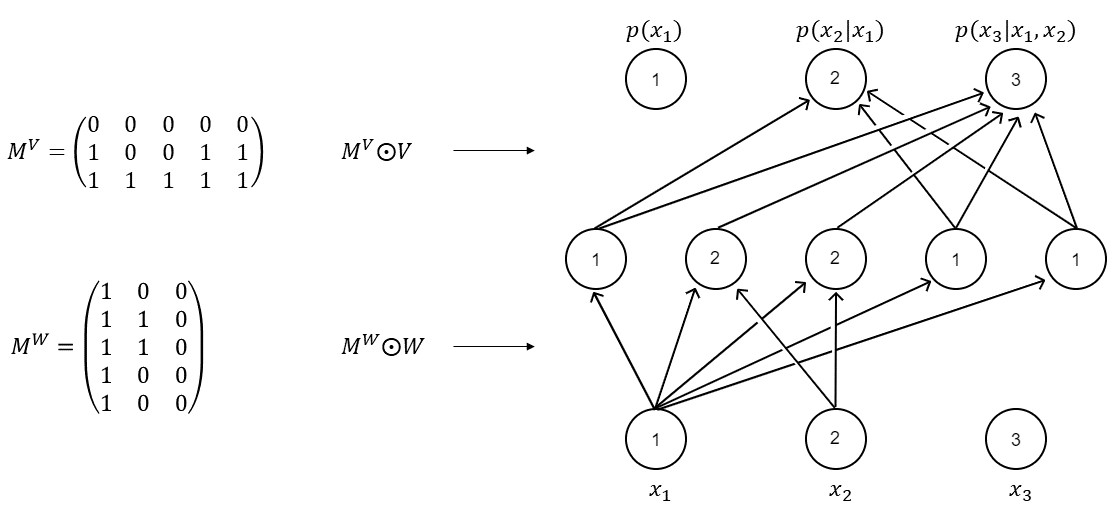
\includegraphics[width=\linewidth]{MADE_vis.jpg}
	\caption[Illustration of MADE]{Illustration of the effect of masking matrices on the graph structure of an autoencoder. The digits inside the hidden layer nodes are the $m(k)$ values that were used to calculate $\mathbf{M}^W$ and $\mathbf{M}^V$, the digits inside input / output nodes indicate the ordering. Connections where the masking matrix is 0 are dropped while others are retained (own figure).}
	\label{fig:MADE}
\end{figure}

\noindent A main disadvantage of MADE is that the order of the conditionals has a large impact on the quality of the learned density. With the correct order it may be possible to learn the density perfectly while for other orders this is not the case. To remedy this, MAF stacks $L$ MADEs and models the random numbers which are used by the MADE in layer $l$ with the model in layer $l+1$ and so on, until the random numbers of the model in the last layer are modeled by a standard Gaussian. Although each individual MADE unit has unimodal conditionals the authors of MAF argue that such a model can learn multimodal conditionals \cite{papamakarios_masked_2017}. According to them, this added flexibility improves model fit.

The central idea behind MAF is, that the distribution to be learned is viewed as a transformation of a base density $\pi_{u} (\pmb{u})$ to the target distribution via a differentiable and invertible transformation $f$. The base density should be simple in the sense that $\pi_{u} (\pmb{u})$ can be easily evaluated for all inputs $\pmb{u}$. For example the standard multivariate Gaussian where $\pmb{u} \sim \mathcal{N}(0, I)$ is a common choice. This means that $f$ takes an input $\pmb{u}$, which follows the base density distribution $\pmb{u} \sim \pi_{u} (\pmb{u})$ and transforms it to data space via the invertible function $\pmb{x}=f(\pmb{u})$. As $f$ is invertible it holds that $\pmb{u} = f^{-1}(\pmb{x})$, and the density $p(\pmb{x})$ can be calculated as

\begin{equation}
	\label{func:maf}
	p(\pmb{x}) = \pi_{u} \bigl(f^{-1}(\pmb{x})\bigr) \biggl\lvert \det \left(\frac{\partial f^{-1}}{\partial \pmb{x}} \right) \biggr\rvert.
\end{equation}

\noindent According to Papamakarios et al. \cite{papamakarios_masked_2017} the computation of this expression is tractable by design. The first part is easy to compute because $f$ is by design invertible and the base density can be evaluated for any input. The absolute determinant of the Jacobian is tractable, because the Jacobian matrix is triangular. This is due to the autoregressive property where the d-th variable $x_d$ only depends on the prior $d-1$ variables $x_{1:d-1}$. Consequently, the Jacobian of $f^{-1}$ is zero for all variables that this variable does not depend on. %TODO: Maybe add further explanation/Terms from og paper.
In each layer the mean and the log standard deviation of the d-th conditional given only the previous previous variables are computed via functions which are implemented as MADE units. Stacking multiple such units on top of each other is possible because if $f_1$ and $f_2$ are differentiable and invertible functions their composition $f_1 \circ f_2$ is also invertible and differentiable. This means the necessary properties to keep expression \ref{func:maf} tractable are maintained, even when stacking multiple layers. The use of masking makes it possible to compute the density $p(\pmb{x})$ of data $\pmb{x}$ in a single forward pass.


\chapter{Related Work}
\label{cha:rel}

While it has been an active research topic for many years, the field of neurosymbolic AI has recently gained renewed traction after calls for more explainable and semantically sound AI systems have gotten louder \cite{garcez_neurosymbolic_2020}. This section gives a concise overview of recent developments in this field and introduces successful models related to the presented work.
Intellectually closest to this thesis is the approach proposed by Rueda et al. \cite{rueda_combining_2019}. They present the idea of using deep neural architectures as the observation model required by CSSMs. In particular the authors use a CNN to learn from time-series sensor data provided by inertial measurement units (IMUs), and predict the observed action class. In that sense the purpose of the system is very similar to the model presented here. The authors evaluated their model on the same carrots data set that will be used for evaluation in this thesis and found that the model performance was comparable to that of state of the art deep models at the time. In the line of this work, a similar approach will be taken. With the difference being, that the observation model is obtained by a neural density estimator like MAF. The benefit of this approach over using a CNN is that MAF actually learns a distribution and can compute the density of sensor data in a single forward pass. While a CNN computes as surrogate the predicted action from sensor data, MAF in fact allows computation of the observation model $p(y_t|x_t)$. Subsequently, this observation model is combined with CCBM to perform probabilistic inference. As the same dataset is used for evaluation in this thesis and the work introduced above, it will be interesting to compare the results with this approach.

Next to this, many other approaches to combine deep neural architectures with symbolic reasoning have been proposed in recent literature. DeepProbLog \cite{manhaeve_deepproblog_2018} is introduced as a framework which combines neural networks and probabilistic-logical modeling via the existing language ProbLog \cite{raedt_problog_nodate}. This is done by extending ProbLog with neural predicates. These special predicates essentially compute the probability of atomic expressions in a probabilistic logic via a neural network. The evaluation of DeepProbLog shows that this framework is capable of performing symbolic reasoning as well as deep learning from examples in an end-to-end fashion. The benefit of this system over previous work is, that it integrates neural networks into a probabilistic-logical framework instead of approximating reasoning with neural nets. Consequently, the resulting model is able to perform probabilistic-logical inference, deep learning and combinations thereof. The downside of this approach is that its inference algorithms and language are ill-suited for dynamic systems, such as HAR.

Another hybrid architecture for HAR in an order-picking scenario is proposed by L\"udtke et al. \cite{ludtke_human_2021}. This model first predicts higher level movement descriptors from sensor data via a temporal convolutional neural network. These attributes are then used by a shallow classifier to estimate the most likely activity class. Additionally, the current process step can be taken into account as context information by making it accessible to the shallow classifier. One main benefit of this system is that it allows the integration of prior context information without re-training the entire network. Consequently, the deep model can be interpreted as a tool for feature extraction from sensor data. This means that it is largely domain independent and only the shallow prediction head has to be adjusted when switching domains. This model is reported to achieve state-of-the-art HAR performance even in the absence of context information, but performance increases further if relevant information from the process step is included, even if it is not always correct.

A very recent approach that shows promising results for HAR is DUSTIN \cite{arrotta_knowledge_2022} which employs knowledge infusion on top of features extracted via a neural network. That is, the model uses a CNN to extract features from time series sensor data as well as the high-level context and concatenates to this representation a set of features which are obtained by a knowledge based reasoner before its classification layer. Just as for CSSMs, this has the added benefit that common-sense knowledge can be introduced to the model, which means that estimated action sequences are consistent with the user-context. However, unlike most models DUSTIN allows infusion of additional knowledge into the deep model itself. That is instead of applying such information before or after the learning process, additional knowledge from a symbolic reasoner is added before the classification layer of the deep model. This is achieved by aggregating raw context data (e.g. the GPS data of the user) to high level context data (e.g. the users semantic location in the world). From this, the symbolic reasoner produces only activities which are consistent with the observed context (e.g. if the user is at a library, they are not doing sports). The evaluation of DUSTIN shows that it is able to outperform other state-of-the-art neuro-symbolic approaches while achieving a high sample efficiency. In comparison with other hybrid approaches that employ knowledge infusion \cite{bettini_caviar_2020, sukor_hybrid_2019}, DUSTIN is the first to apply the knowledge infusion within the deep model for the task of recognizing human activities.


\chapter{Methods}
\label{cha:alg}

At its core, the hybrid model proposed in this paper consists of three main components which can be exchanged with other methods and combined in a modular way. Figure \ref{fig:schema} illustrates a schematic of these components and their interactions. Ultimately, the goal of the hybrid model is to achieve sate of the art HAR performance with increased sample efficiency compared to approaches which solely rely on deep learning methods. To this end three components are defined which can be altered to investigate the effects of each component.

\begin{figure}[h]
	\centering
	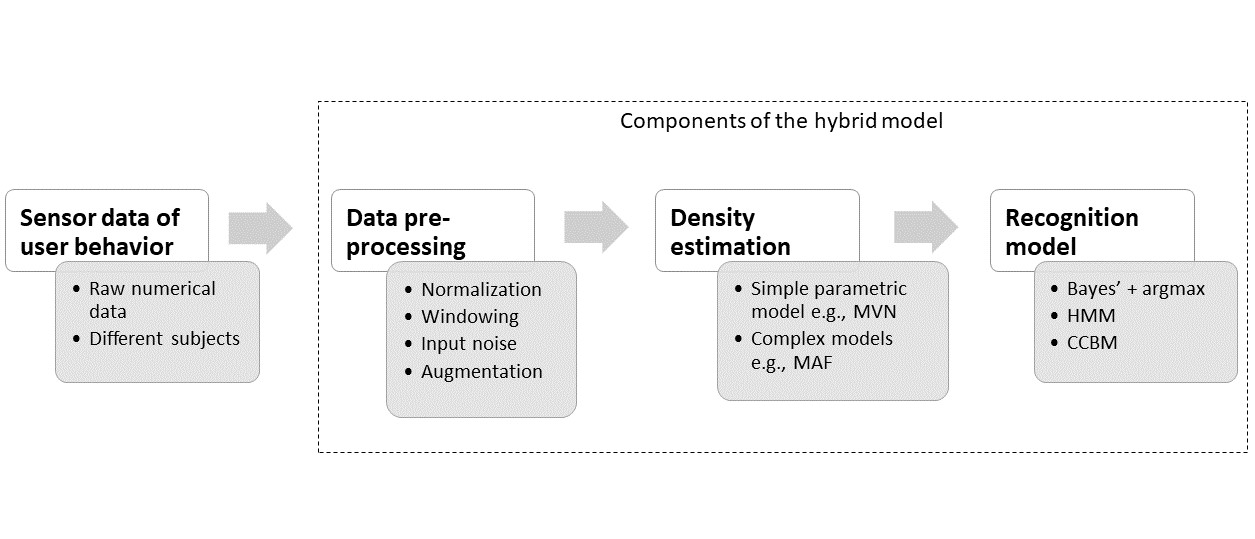
\includegraphics[width=\linewidth]{Hybrid_schmeatic.jpg}
	\caption[Hybrid architecture components]{Components of the hybrid architecture and some of their possible variations (own image).}
	\label{fig:schema}
\end{figure}

\noindent First is the data pre-processing stage in which numerical raw data is read and processed. Various steps can be undertaken here to make the training of the following module more robust. Secondly, a method for density estimation is employed to obtain sample densities. The third an last step in this process is the recognition model which may use the obtained densities directly for activity recognition or as an observation model for more complex models. From this the concrete prediction of a activity class or state is obtained. The remainder of this chapter introduces each component and the implementation thereof in greater detail. Furthermore, some other models choices for these components are discussed briefly.

\paragraph{Data pre-processing}
The data of all three datasets used in this work stems from inertial measurement units (IMUs) which measure acceleration and angular rates. MotionSense \cite{malekzadeh_mobile_2019} and the UCI HAR \cite{anguita_public_2013} dataset use the accelerometer and gyroscope sensors of smartphones, while the Carrots dataset \cite{kruger_recognising_2011} uses standalone IMUs which are located in 5 different locations on the body. Furthermore, the UCI HAR dataset has pre-computed features while the remaining two contain raw sensor data.

In terms of pre-processing several steps were undertaken and their effects are evaluated in section \ref{sec:results} of this thesis. To facilitate an evaluation that is as close to a real world scenario as possible, a leave-one-subject-out strategy was employed for splitting the data into test and training set. Realistically, the model would be trained on some data and each new subject would not have its data in the training set. This fact is emulated by leaving one or more subjects completely out of the training set and using this subject for testing. This strategy was employed for the Carrots and MotionSense datasets, for the UCI HAR dataset the predefined train-test split was used which also leaves a set of subjects completely out of the training set. Additionally, each channel in the data is normalized to the interval $[0,1]$. This is achieved by fitting a \emph{MinMaxScaler} to the training data, the same transformation with this scaler is then applied to the test data to normalize it in the same way. Furthermore, three optional pre-processing steps may be employed for the Carrots and MotionSense datasets. These steps are windowing, augmentation, and noise addition. Windowing segments the raw data into windows of a specified window size \emph{T}, with a step size of \emph{s} indicating by how many samples to step the subsequent window. Note, that window size and step size can be used to create overlapping windows. If \emph{T} is the same as \emph{s} no overlap occurs, if for example $s = \frac{T}{2}$, subsequent windows have an overlap of 50 \%. Such overlap creates more samples than windowing without it. The class of a window is the majority class of its components. It is apparent that with a window size of $T=1$ the notion of a sample (i.e., an example at a single time step) and a window agree. For simplicity, a data window of arbitrary size will be referred to as a \emph{sample} in the remainder of this thesis.

The idea behind windowing the data is that actions in reality have a duration that is typically much greater than the sampling rate of the sensors. Thus, many individual time steps can be segmented together in order to obtain a sample which corresponds to a real-world activity. This is typically done for HAR applications. Since the UCI HAR dataset is already segmented into windows of size $T=128$ this option is not applicable to that dataset. Next to this, two simple data augmentation methods can be used to augment the training data. These are adapted from a paper on data augmentation for sensors by Um et al. \cite{um_data_2017}. Namely scaling and jittering of data. If used, a proportion of the training data, i.e., from 0 to 100 \% is added to the original data in a slightly altered fashion to increase the number of training samples. The employed augmentation methods are jittering, that is adding Gaussian noise with $\mu = 0, \sigma = 0.05$, and scaling, that is scaling each channel by multiplying with a factor drawn from a normal distribution with $\mu = 1, \sigma = 0.1$. This step was added as an option because the amount of training data is often very limited. To combat overfitting of the subsequent MAF module another option was introduced: Adding noise directly to the raw data. If this option is set, Gaussian noise with $\mu = 0, \sigma = 0.025$ is added to training samples. The idea here is, that this does not change the samples enough to where they would be considered a different class, but enough that some of the interpersonal variability between how different subjects perform certain activities is captured. Adding noise differs from the data augmentation option where the original data is left unchanged and only augmented samples are added to the training data. It is also possible to use both mechanisms at the same time. Both of these options are applicable to the Carrots and MotionSense datasets. UCI HAR is already pre-processed and has pre-computed features. It was thus chosen not to employ any methods that alter this default pre-processing of the UCI HAR dataset.

One of the main difficulties of HAR lies in the fact that different subjects often produce greatly differing sensor readings for the same activity, that is a high intra-class variability. This is a consequence of various physiological differences between subjects. Factors such as variances in age, height or weight can impact how actions are performed, and thus sensor readings, strongly. Consequently, it is preferable for HAR tasks to have a dataset that captures most of this variability in its training set by containing data of many different subjects. However, labeled motion data is often hard to obtain. To counteract this, the pre-processing component of the hybrid model could be refined further. For example, more advanced augmentation methods, such as the ones proposed by Um et al. \cite{um_data_2017}, are available. These aim to combat a lack of labeled data. Furthermore, representation learning from unlabeled time series in a self-supervised manner as proposed by Eldele et al. \cite{eldele_time-series_2021} may be an interesting research direction. In this way helpful representations may be learned which are useful for the downstream task of recognizing human activities.


\paragraph{Density estimation}
The second component of the proposed hybrid system is the density estimation component. This module computes the probability density of samples which can be used later on in the recognition model either to build the observation model or to predict actions from conditional densities directly. Just like the other two modules, many concrete implementations are plausible for this component. Potentially the simplest method is a simple parametric model for which the probability densities can be computed easily. An example of this is the multivariate normal (MVN) distribution. For this thesis one MVN per activity class $y$ was fitted for benchmarking purposes. Thus a set of MVNs with unconstrained covariance matrices allow conditional density estimation. Each MVN can be used to obtain the density $p(\pmb{x}|y)$ of a sample.

However, there are more sophisticated methods of obtaining probability densities from samples. One such method is density estimation based on neural networks such as the previously discussed MADE/MAF models. The goal of the neural architecture of the hybrid system is to obtain a likelihood from given sensor data which is useful for the downstream task of recognizing human activities. At its heart, MAF is trained on data to fit the assumed true data distribution from samples. As discussed in section \ref{sec:maf}, MAF calculates densities of samples within a single forward pass, which makes obtaining densities with a trained MAF computationally inexpensive. At test time this allows to take a set of samples and produce for each of those samples the likelihood of the observed data. For reasons of numerical stability during training and testing, the log likelihood (natural logarithm) is used in this work. It is important to note here, that obtaining a single density from a sample is not yet what we want to achieve. The final goal of MAF in this use case is to obtain the observation model from it. For this the likelihood of observed sensor data given the system state should be computed. To achieve this, MAF is adapted to be conditioned on the additional class information $y$ of each example. That is, from the set of labeled training pairs $p(\pmb{x}|y)$ can be computed instead of computing $p(\pmb{x})$. According to Papamakarios et al. \cite{papamakarios_masked_2017} this extension to handle class information $y$ comes naturally in MAF. It is obtained by conditioning each term in the chain rule decomposition of the joint probability on the available class information $y$. This means that $p(\pmb{x}|y)$ decomposes into $p(\pmb{x}|y) = \prod_{i}^{} p(x_i|x_{1:d-1},y)$. The additional class information is added to the input as a one hot encoded class vector. This information is then used by each layer as an additional input to the raw data, as the class information is always given at every time step no connections need to be masked from the class inputs to the remainder of the network, as this does not violate the autoregressive property. For this work conditional MAF was employed exclusively, since all of the three datasets used for evaluation contain labeled data, and conditional MAF was shown to significantly outperform unconditional MAF if labeled data is available \cite{papamakarios_masked_2017}. To build this model a base implementation of MAF in PyTorch \cite{kostrikov_pytorch-flows_2022} was used and heavily adapted to fit the requirements of this thesis. Each Layer of the MAF consists of a MADE followed by a Batch normalization layer. The MADE uses the ReLu activation function. The number of MAF modules that are stacked on top of each other is a tunable hyperparameter. However, five blocks of the above architecture provided the most promising results in many of the experiments.

MAF is trained by minimizing the negative log likelihood (NLL) loss, over a number of max epochs which can be set as a hyperparameter. The best model is selected by the lowest loss on the validation data. Since, the downstream task is the goal of recognizing activities it was also tested to select the best model according to recognition accuracy. However, in most cases these two methods of selecting the best model agree or differ only marginally. Therefore, minimizing the NLL loss was chosen as a suitable mechanism for model selection. Furthermore, it is important that training samples are shuffled to ensure that they are independent and identically distributed. If this is not done, most batches only contain samples from one class and MAF tends to learn unimodal or other very simple distributions.

In theory other generative models can be employed in a very similar fashion to obtain (conditional) densities of samples. Another notable example that can be used for density estimation and is also based on invertible flows is Real NVP \cite{dinh_density_2017} or extensions thereof like Glow \cite{kingma_glow_2018}.

\paragraph{Recognition model}
The last component of the proposed hybrid model is the recognition model. The goal of this model is to accurately recognize human activities given the output of the previous step. To achieve this, many concrete options are applicable. The following paragraph will introduce
At test time the set of test samples is passed through the MAF and the $\log p(\pmb{x}|y)$ of each sample is computed. To obtain a prediction of activities from these densities we calculate the log density conditioned on each class $c \in C$ and then use Bayes theorem as a simple classifier on top. Hence we get the $\log p(\pmb{x}|y_c)$ for class c with a single forward pass through the MAF. By doing this for all classes we obtain a matrix containing as rows the number of test samples and for each test sample the logarithmic density of that sample for each of the classes as columns. From there Bayes' theorem is used to calculate $p(y_c|\pmb{x}) = \frac{p(\pmb{x}|y_c) \cdot p(y_c)}{p(\pmb{x})}$, as $p(\pmb{x})$ is the same within each sample $\pmb{x}$, the denominator is a constant factor per row thus we achieve a proportional result which suffices for predicting the most probable class. The prior $p(y_c)$ for all classes $c$ is easily computed as the class distribution of training samples. As we operate in log space the numerator of Bayes' theorem is obtained by adding the values $\log p(\pmb{x}|y_c) + \log p(y_c)$. Thus we obtain a result that is proportional to $p(y_c|\pmb{x})$ for all classes. Consequently, we predict the most probable class by getting the $argmax$ over all classes y.


%\begin{algorithm}{\MYCALL{EfficientLOD}{$\ALI$, $\ONT_1$, $\ONT_2$}}
%\caption[Efficient Local Optimal Diagnosis]{}
%\label{alg:efficient-lod}
%\begin{algorithmic}[1]
%% \STATE $\ALI' \leftarrow \ALI$
%% \STATE $k \leftarrow 0$
%\LOOP
%	\FOR{$i \leftarrow k$ to  $\left|\ALI'\right| - 1 $}
%		\FOR{$j \leftarrow 0$ to $i - 1$}
%			\IF{\MYNOT \MYCALL{PossiblyCoherentPair}{$\ALI'[j]$,  $\ALI'[i]$, $\ONT_1$, $\ONT_2$}}
%				\STATE $\ALI' \leftarrow \ALI' \setminus \{\ALI'[i]\}$
%				\STATE $i \leftarrow i -1$ \ \algorithmiccomment{adjust $i$ to continue with next element of $\ALI'$}
%				\STATE \MYBREAK \ \algorithmiccomment{exit inner for loop}
%			\ENDIF
%		\ENDFOR	
%	\ENDFOR
%	\STATE $k \leftarrow$ \MYCALL{SearchIndexOfAccusedCorrespondence}{$\ALI'$, $\ONT_1$, $\ONT_2$}
%	\IF{$k = \MYNIL$}
%		\RETURN $\ALI \setminus \ALI'$
%	\ENDIF
%	\STATE \algorithmiccomment{let $k^*$ be the counterpart of $k$ adjusted for $\ALI$ such that $\ALI[k^*] = \ALI'[k]$}
%	\STATE $\ALI' \leftarrow \ALI'[\ldots k-1] \cup \ALI[k^*+1 \ldots]$ 
%\ENDLOOP
%\end{algorithmic}
%\end{algorithm}

\chapter{Experimental Evaluation}
\label{cha:exp}

\section{Datasets}
\label{sec:data}
The three datasets used in this evaluation are the Carrots dataset \cite{kruger_recognising_2011}, MotionSense \cite{malekzadeh_mobile_2019} and the UCI HAR dataset  \cite{anguita_public_2013}. All three datasets contain measurements from IMUs. The individual datasets are introduced in greater detail in the paragraphs below.
\paragraph{Carrots}
The Carrots dataset uses standalone IMUs which are attached to the subjects body in five locations: upper body, left forearm, right forearm, left calf, right calf. The data stems form seven subjects which were tasked with a typical activity of daily living. Namely, the execution of preparing and having a meal: preparing the ingredients, cooking, serving the meal, having a meal, cleaning the table, and washing the dishes. The dataset consists of the raw acceleration and angular rates that were recorded with motion capturing system based on wearable inertial measurement units (IMUs). It contains 16 action classes which are annotated and are used as the labels in this work. The data is recorded at a sampling rate of 120 Hz. To follow the leave one-subject out validation it was decided arbitrarily that subject 7 would be the test subject and the remaining subjects would be used for training and validation. Each sensor at each of the five locations records the angular rate and acceleration in x,y and z direction. Thus the dataset consists of $D = 5 \cdot 6 = 30$ channels. The training set contains $N=143086$ smaples and the test set $30427$.

\paragraph{MotionSense}
The MotionSense dataset includes time-series data generated by accelerometer and gyroscope sensors. Attitude, gravity, acceleration, and rotation rate on the x,y and z axis. Consequently this dataset has $D = 4 \cdot 3 = 12$ channels. The data is collected with an iPhone 6s kept in the front pocket of the subject using SensingKit which collects information from Core Motion framework on iOS devices. All data is collected at a 50 Hz sample rate. A total of 24 participants in a range of gender, age, weight, and height performed 6 activities in 15 trials in the same environment and conditions: downstairs, upstairs, walking, jogging, sitting, and standing. The training data contains $N=1638432$ samples. 

\paragraph{UCI HAR}
The UCI HAR dataset is slightly different because it is already processed and contains pre-computed features. The experiments have been carried out with a group of 30 volunteers within an age bracket of 19-48 years. Each person performed six activities wearing a smartphone (Samsung Galaxy S II) on the waist. Using its embedded accelerometer and gyroscope, we captured 3-axial linear acceleration and 3-axial angular velocity at a constant rate of 50Hz. The experiments have been video-recorded to label the data manually. The obtained dataset has been randomly partitioned into two sets, where 70 \% of the volunteers was selected for generating the training data and 30 \% the test data.

The sensor signals (accelerometer and gyroscope) were pre-processed by applying noise filters and then sampled in fixed-width sliding windows of 2.56 sec and 50 \% overlap. The sensor acceleration signal, which has gravitational and body motion components, was separated using a Butterworth low-pass filter into body acceleration and gravity. The gravitational force is assumed to have only low frequency components, therefore a filter with 0.3 Hz cutoff frequency was used. From each window, a vector of features was obtained by calculating variables from the time and frequency domain.


\section{Settings}
\label{sec:setting}
The experiments were conducted with five MAF layers stacked on top of each other, batch size is $bs = 128$, the number of hidden neurons in each MADE Layer is $H=512$, the learning rate was set to $5 \times 10^{-5}$ and weight decay of the Adam optimizer to $1 \times 10^{-6}$. Other notable hyperparameter settings are reported individually in each results table.


\section{Experiments}
\label{sec:exp}


\section{Results}
\label{sec:results}


%\begin{table}[h]
%
%\begin{center}
%\begin{tabular*}{\textwidth}{@{\extracolsep{\fill}}>{\scriptsize}l|>{\scriptsize}c>{\scriptsize}c>{\scriptsize}c|>{\scriptsize}c>{\scriptsize}c>{\scriptsize}c>{\scriptsize}c} 
%& \multicolumn{3}{>{\scriptsize}c|}{Baselines} & \multicolumn{4}{>{\scriptsize}c}{Decision Tree} \\\hline
%Ontology & M(edian) & G(ood) & E(vil) & results & $\Delta$-M & $\Delta$-G & $\Delta$-E \\\hline\hline
%\#301 & 0.825 & 0.877 & 0.877 & 0.855 & +0.030 & -0.022 & -0.022 \\\hline
%\#302 & 0.709 & 0.753 & 0.753 & 0.753 & +0.044 & +0.000 & +0.000 \\\hline
%\#303 & 0.804 & 0.860 & 0.891 & 0.816 & +0.012 & -0.044 & -0.075 \\\hline
%\#304 & 0.940 & 0.961 & 0.961 & 0.967 & +0.027 & +0.006 & +0.006 \\\hline
%\bfseries Average & \bfseries 0.820 & \bfseries 0.863 & \bfseries 0.871 & \bfseries 0.848 & \bfseries +0.028 & \bfseries -0.015 & \bfseries -0.023 
%
%\end{tabular*}
%\caption[Good vs. Evil]{Comparison between the Good and the Evil}
%\label{tab:confonly}
%\end{center}
%\end{table}

\begin{table}
\tiny
\begin{tabularx}{\textwidth}{llrrllrrrr}
	\toprule
	Dataset &  W &  T &  s &  A &  N &    MVN LL &    MAF LL &  MVN ACC &  MAF ACC \\
	\midrule
	CARROTS &   False &       0 &       0 &    False &  False &   63.0739 &   68.2259 &   0.6006 &   0.5384 \\
	CARROTS &   False &       0 &       0 &    False &   True &   56.7594 &   59.6865 &   0.5932 &   0.6037 \\
	CARROTS &   False &       0 &       0 &     True &  False &   52.1412 &   68.1716 &   0.5683 &   0.5624 \\
	CARROTS &   False &       0 &       0 &     True &   True &   45.6814 &   59.1802 &   0.5103 &   0.6166 \\
	CARROTS &    True &      26 &      13 &    False &  False & 2986.2914 & 1555.2181 &   0.3299 &   0.3290 \\
	CARROTS &    True &      26 &      13 &    False &   True & 2016.7640 & 1416.1207 &   0.4398 &   0.3861 \\
	CARROTS &    True &      26 &      13 &     True &  False & 1881.0891 & 1720.2389 &   0.4312 &   0.4121 \\
	CARROTS &    True &      26 &      13 &     True &   True & 1566.8524 & 1513.4050 &   0.4909 &   0.5351 \\
	CARROTS &    True &       8 &       4 &     True &  False &  530.5136 &  695.9487 &   0.3759 &   0.5341 \\
	CARROTS &    True &      64 &      32 &     True &  False & 1375.9667 & 3319.6480 &   0.1215 &   0.4030 \\
	UCIHAR &    True &       0 &       0 &    False &  False &  717.9488 &  351.7945 &   0.9444 &   0.6291 \\
	\bottomrule
\end{tabularx}
\end{table}

\begin{table}
	\tiny
	\begin{tabularx}{\textwidth}{llrrllrrrr}
		\toprule
		Dataset &  W &  T &  s &  A &  N &    MVN LL &    MAF LL &  MVN ACC &  MAF ACC \\
		\midrule
		MOSENSE &    True &     128 &      64 &    False &  False & -242.2431 & 1264.8010 &   0.4966 &   0.7487 \\
		MOSENSE &    True &     128 &      64 &    False &   True &  435.8816 & 1200.5637 &   0.6580 &   0.8254 \\
		MOSENSE &    True &     128 &      64 &     True &  False &  587.4257 & 1582.0021 &   0.6731 &   0.8030 \\
		MOSENSE &    True &     128 &      64 &     True &   True &  210.0161 & 1284.2458 &   0.6544 &   0.7916 \\
		MOSENSE &    True &      64 &      32 &     True &   True &  579.2101 &  868.5525 &   0.8166 &   0.8046 \\
		MOSENSE &    True &      32 &      16 &     True &   True &  289.0209 &  516.7429 &   0.7376 &   0.7864 \\
		UCIHAR &    True &       0 &       0 &    False &  False &  846.4878 & 1256.1664 &   0.9474 &   0.8792 \\
		UCIHAR &    True &       0 &       0 &    False &   True &  846.4878 &  868.8217 &   0.9474 &   0.9433 \\
		\bottomrule
	\end{tabularx}
	\caption{\label{tab:eps50} Log likelihoods and prediction accuracies of MAF and a baseline multivariate normal distribution trained per class with unconstrained covariance matrix. The Settings of the experiments are reported in the first 6 columns, the results in the remaining four. MAF was trained for a maximum of 50 epochs with the settings described above.}
\end{table}




\chapter{Conclusion}
\label{cha:conclusion}


\section{Summary}
\label{sec:sum}


\section{Future Work}
\label{sec:future}


\bibliographystyle{plain}
\bibliography{thesis-ref}


\appendix

\chapter{Program Code / Resources}
\label{cha:appendix-a}

The source code, a documentation, some usage examples, and additional test results are available at ...

They as well as a PDF version of this thesis is also contained on the CD-ROM attached to this thesis.

\chapter{Further Experimental Results}
\label{cha:appendix-b}

In the following further experimental results are ...


\newpage


\pagestyle{empty}


\section*{Ehrenw\"ortliche Erkl\"arung}
Ich versichere, dass ich die beiliegende Master-/Bachelorarbeit ohne Hilfe Dritter
und ohne Benutzung anderer als der angegebenen Quellen und Hilfsmittel
angefertigt und die den benutzten Quellen w\"ortlich oder inhaltlich
entnommenen Stellen als solche kenntlich gemacht habe. Diese Arbeit
hat in gleicher oder \"ahnlicher Form noch keiner Pr\"ufungsbeh\"orde
vorgelegen. Ich bin mir bewusst, dass eine falsche Er- kl\"arung rechtliche Folgen haben
wird.
\\
\\

\noindent
Mannheim, den 31.09.2022 \hspace{4cm} Unterschrift

\end{document}
